{\color{blue}2-25} %We continue the discussion of convexity of pressure.}

\subsection{Convexity of the pressure and its implications}

\begin{thm}[H\"older inequality]
For any pair of functions $f,g:\Omega\to \mathbb{R}$ on a (positive) measure space, for $\frac{1}{p}+ \frac{1}{q}=1$,
%use different symbols, but that's life.
\[
\left| {\int f(\omega) g(\omega) \,d\mu(\omega)} \right| \le \int \left[ {\int |f|^p \,d \mu} \right]^{\frac{1}{p}} \left[ {\int |g|^q\,d\mu} \right]^{\frac{1}{q}}.
\]
\end{thm}
This can be proved using Jensen's inequality.

\begin{thm}
For any function $\phi:\Omega\to \mathbb{R}$, 
\[
P(h) = \ln \int e^{h\phi(\omega)}\,d\mu(\omega)
\]
is convex in $h$.
%good to see another proof
\end{thm}
\begin{proof}[Proof 1]
Differentiate:
\begin{align*}
P'(h) &=\left\langle {\phi}\right\rangle_h\\
P''(h)&=\left\langle {(\phi-\left\langle {\phi_h}\right\rangle)^2}\right\rangle_h\ge 0.
\end{align*}
\end{proof}
\begin{proof}[Proof 2]
Let $h_t=th_0+(1-t)h_1$. Then
\begin{align*}
\int e^{h_t\phi} \,d\mu &= \int (e^{h_0\phi})^t (e^{h_1\phi})^{1-t}\,d\mu \\
&\le \left( {\int e^{h_0}\,d\mu} \right)^t \left( {\int e^{h_1}\,d\mu} \right)^{1-t}.
\end{align*}
Hence 
\[
P(h_t) \le tP(h_0) + (1-t) P(h_1).
\]
%regardless of differentiability properties. Never assume differentiability of $\phi$.
\end{proof}
Note the proof doesn't assume differentiability of $\phi$.
%The pressure is differentiable in its arguments. 

We used the density for fluctution estimates. %not complicated, but prepare.

Our goal is to estimate 
\begin{align*}
\mathbb{P}(H(\sigma)\le \left\langle {H}\right\rangle_\beta - \varepsilon |\Lambda|)
&=\int_{\Omega_\Lambda} \mathbbm{1}[H(\sigma)\le \left\langle {H}\right\rangle_\beta - \varepsilon |\Lambda|] \frac{e^{-\beta H_\Lambda(\sigma)}\,\rho_0(d\sigma)}{Z_{\Lambda}(\beta)}.
\end{align*}
We use the bound 
\[
\mathbbm{1}[H\le \left\langle {H}\right\rangle-\varepsilon |\Lambda|] \le e^{-tH} e^{t\left\langle {H}\right\rangle - \varepsilon|\Lambda|}.
\]
Then 
\begin{align*}
\mathbb{P}(H(\sigma)\le \left\langle {H}\right\rangle_\beta - \varepsilon |\Lambda|)
&\le \left[ {\int_{\Omega_\Lambda} e^{-tH}\rho_{\beta}(\sigma)} \right] e^{t(\left\langle {H}\right\rangle-\varepsilon|\Lambda|)}\\
&= \frac{Z(\beta+t)}{Z(\beta)}e^{t(\left\langle {H}\right\rangle-\varepsilon|\Lambda|)};
\end{align*}
we got the partition temperature at shifted temperature.
The partition function is a generating function: its derivative up to sign gives energy,
\begin{align*}
\psi(\beta) &= \frac{1}{|\Lambda|}\ln \underbrace{\left[ { \int e^{-\beta H_\Lambda} \rho_0(d\sigma)} \right]}_{Z_{\Lambda}(\beta)}\\
\left\langle {H}\right\rangle_\beta &= -\psi_A'(\beta) |\Lambda|.
\end{align*}
Using this, we get
\begin{align*}
\mathbb{P}(H(\sigma)\le \left\langle {H}\right\rangle_\beta - \varepsilon |\Lambda|)&\le 
\frac{Z(\beta+t)}{Z(\beta)}e^{-t[\psi'(\beta)+\varepsilon]|\Lambda|}\\
&\le \frac{e^{\psi(\beta+t)|\Lambda|}}{e^{(\psi(\beta) + [\psi'(\beta) + \varepsilon]t)|\Lambda|}}.%how to get this step?
\end{align*}
%pressure as function of inverse temperature is convex.
Thinking of $\psi$ as a function of inverse temperature $\beta$, $\psi$ is convex. The slope at a point is $\psi'(\beta)$. In the denominator is a linear function which is equal to $\psi(\beta)$ at $\beta$ but increases a bit faster than the tangent line.

By convexity, for all $\varepsilon>0$, $t>0$ small enough, % there exists $t(\ep), \de(\ep)>0$ such that
\[
\psi(\beta) + t_\varepsilon [\psi'(\beta) + \varepsilon] - \psi(\beta+t) \ge 0
\]
Pick $t$ to maximize this difference. Denoting $\delta(\varepsilon)=\sup_{t>0}\delta(t)$ we have
\[
\mathbb{P}_\beta (H_\Lambda\le \left\langle {H_{\Lambda}}\right\rangle - \varepsilon|\Lambda|) \le e^{-\delta (\varepsilon)|\Lambda|}.
\]

\begin{center}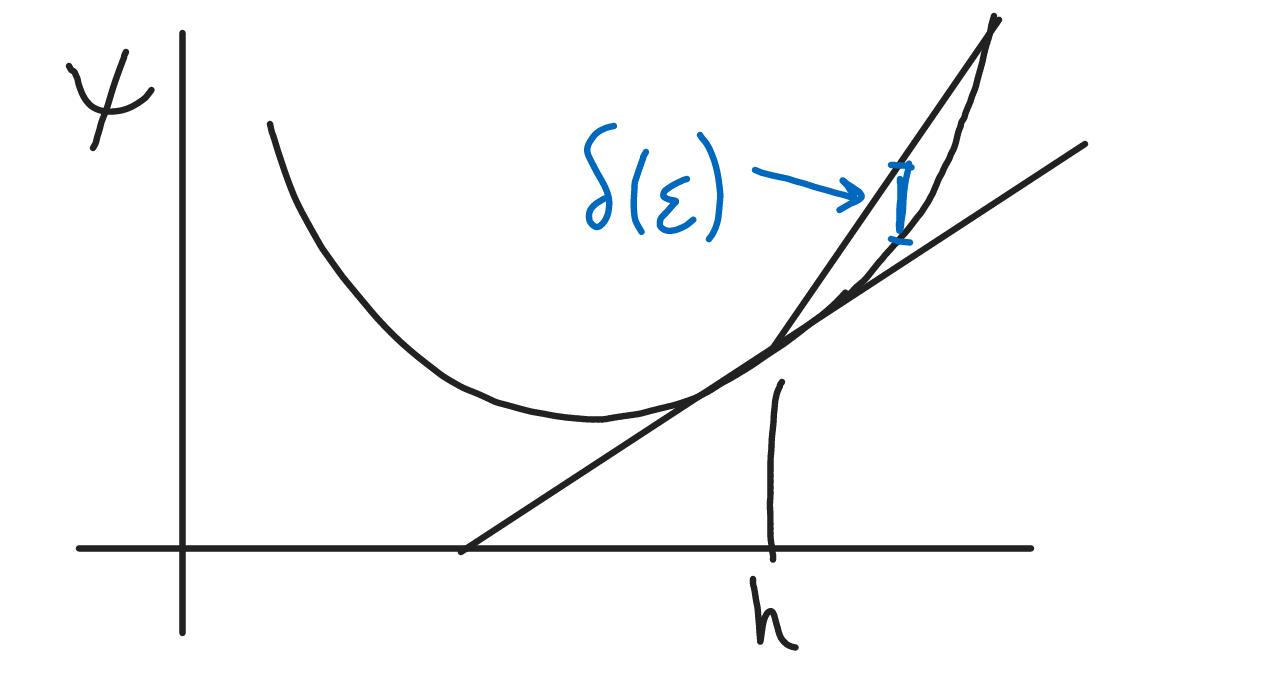
\includegraphics[scale=.25]{images/9-1}\end{center}

The probability that the energy density falls by $\varepsilon$ below its mean decays exponentially. This is the kind of decay we were talking about with large deviation principles.
Similarly we can show 
\[
\mathbb{P}_\beta (H\ge \left\langle {H}\right\rangle + \varepsilon|\Lambda|) \le e^{-\delta_+ (\varepsilon)|\Lambda|}.
\]
%kettle on the floor.
%kettle on the table
This is left as an argument. 
We can repeat the argument, or apply what we proved to a system where the Hamiltonian is the negative.

The convex functions converge to a convex function. %Since $f$ converges pointwise, we can conclude from the convexity of the limiting function, 
%finite vs. infinite systems not so obvious. 
In the infinite volume limit, the function may not be differentiable, but the left and right derivatives exist. Our argument is really comparing with the slope of the function coming from above; for the other inequality, compare with the slope of the function from below.

Since the pressure converges, 
%REC
you can conclude that given a van Hove sequence, for $\Lambda$ large enough, you can conclude the bounds (not optimally) with $\delta/2$. 

\subsection{Large deviation principle for van Hove sequences}

\begin{thm}
Assume that the infinite volume pressure $\psi$ is differentiable at $\beta_0$. Then for all $\Lambda_n\uparrow \mathbb{Z}^d$ (in the van Hove sense). %don't have to be cubes. suface-to-volume goes to 0.
Then for any $\varepsilon$, there is $N<\infty$ such that for all $n\ge N$, 
\[
\mathbb{P}_{\beta, \Lambda_n}\left( {\left| {\frac{1}{|\Lambda|}H_\Lambda(\sigma) + \psi'(\beta)} \right|\ge \varepsilon} \right)\le e^{-\frac{\delta(\varepsilon)}{2}|\Lambda|}.
\]
\end{thm}
If the infinite volume pressure is differentiable at a particular $\beta$, then in large enough finite volume, then the fluctuations per volume is small. with high probability. 
%corridor of small width, eventually finite volume pressures with $\ep$ of that. Half of that gap is realized. $\de(\ep)$ is read from the infinite value limit function. 
Look at the infinite volume function; for every $\varepsilon$, ask when we move right (left) at $\varepsilon$ greater (less) than the slope, how far we move to have the largest discrepancy. Wait for the gap between the infinite and finite volume case function to be less than half. 

So far we studied the distribution of the energy. But you may want to know the distribution of other quantities such as magnetization, spin, and number of clusters of a certain class. These are covered by the same analysis except you consider the dependence of the free energy. 

{\color{red}TODO: edit}
What is the physical implication for a lattice model? If you know the pressure as a function of inverse temperature. Pressure is a thermodynamic function. We are interested in sysm of deg ... tell us something... typical range of values of the energy of this configuration. At places where the energy is differentiable, the total energy per unit volume does not fluctuate much. We expect $\sqrt{}$ volume of fluctuations. This is like CLT for nonindependent variables.
%tiny $\ep$ times the volume. 
%REC


What happens if the pressure is not differentiable?
Without assuming differentiability of $\psi(\beta)$, we have 
\begin{align*}
\mathbb{P}_{\beta,\Lambda} \left( {\frac{1}{|\Lambda|} H \ge \psi'(\beta+0) + \varepsilon} \right)&\le e^{-\frac{\delta(\varepsilon)}{2}|\Lambda|}\\
\mathbb{P}_{\beta,\Lambda} \left( {\frac{1}{|\Lambda|} H \le  \psi'(\beta-0) -\varepsilon} \right) &\le e^{-\frac{\delta(\varepsilon)}{2}|\Lambda|}.
\end{align*}
(Note $\psi'(\beta-0)\le \psi'(\beta+0)$.) To extend to the densities of other local observables,
\[
H(\sigma) = \sum_{A\subseteq \mathbb{Z}^d} J_A \phi_A(\sigma)
\]
with $J_A = J_{S_n}A$ for all shifts $S_n$. 
(The proper way to do this is to introduce coupling constants depending on the equivalence class of terms modulo translation. For example, Ising coupling has 2 parameters corresponding to nearest neighbor coupling and external field.)

For a collection of translation-invariant interactions, we denote 
\[
\psi(\beta,J) = \lim_{\lambda \uparrow \mathbb{Z}^d} \frac{1}{|\Lambda|} \ln Z_{\Lambda}(J,\phi).
\]
\begin{thm}\label{thm:j-limit}
For any translation-invariant interaction with $\left\Vert {J}\right\Vert<\infty$, %$\phi$ with $\ve{\phi}<\iy$, 
the limit 
$
\psi(\beta, J) 
$
exists and is a convex function of $J$ (it is jointly convex in all parameters). 
\end{thm}
We think of pressure as a function of both the temperature and parameters such as the magnetic field.
%notation is not consistent.
%Banach space notation...
For example, for $H=-J\sum_{\{x,y\},|x-y|=1} \sigma_x\sigma_y - h\sum_x \sigma_x$, %infinitely many terms but 2 paramters. 
$\psi$ is a function $\psi(\beta, J,h)$. We have
\[
\frac{\partial \psi_{\Lambda}}{\partial h} = \beta\left\langle { \frac{1}{|\Lambda|}\sum_{x\in A} \sigma_x}\right\rangle.
\]
and
\begin{align*}
\psi_{\Lambda}(\beta, J, h) &= \frac{1}{|\Lambda|} \ln \int e^{\beta(J\sum_{\left\langle {x,y}\right\rangle} \sigma_x\sigma_y+ h\sum_{x\in A} \sigma_x)}\rho_0(d\sigma)\\
\psi(\beta,J) &= \lim_{\Lambda\uparrow \mathbb{Z}^d} \frac{1}{|\Lambda|}\ln Z_{\Lambda}(J\phi)
\end{align*}
%jointly convex is almost everywhere diffble
%regardless whether continuous, can sandwich typical values within the left and right derivatives. 
%\begin{thm}
%For any $\phi$ with $\ve{\phi}<\iy$, $\psi(\be,J)$ is jointly convex in $J$.
%\end{thm}
Introduce as many parameters as you think are relevant.

In the homework, you will look at the simplest system, ideal gas. There are no interactions. We introduce something akin to the magnetization. Compute the pressure for an ideal gas and use this to compute the entropy of the system. The Legendre transform allows you to read the ... from the free energy. You'll learn how to arrive at this celebrated formula 
\[
-\rho\ln \rho + (1-\rho)\ln (1-\rho).
\]
It becomes a challenge to evaluate partition functions and find their singularities. Ising calculated the partition function for the 1-D model; you will do the calculation too. He said it has no singularity. If you move to 2 dimensions, it does exhibit a phase transition. %Initial people we wrong.
The 2-D model is solvable by other techniques.